%------------------------------------------------------------------------------------------------
%Algorithmen
%------------------------------------------------------------------------------------------------
\section{Algorithmen}
\subsection{Eigenschaften - Zwingende Forderungen}
\begin{itemize}
	\item Korrektheit
	\item Finitheit: Eindeutige Beschreibbarkeit
	\item Determiniertheit: Erzielt bei gleichen Vorbedingungen immer dasselbe Resultat
	\item Determinismus: N"achster Schritt zu jedem Zeitpunkt bekannt
	\item Effizienz 
	\item Einfachheit/Verst"andlichkeit
\end{itemize}

\subsection{Eigenschaften - Optionale Forderungen}
\begin{itemize}
	\item Effizienz 
	\item Einfachheit/Verst"andlichkeit
\end{itemize}

\subsection{Beschreibungsmethoden}
\begin{itemize}
	\item Aktivitätsdiagramm
	\item Konkrete Programmiersprache
	\item Pseudocode
	\item UML
\end{itemize}

\subsection{Korrektheit}
Kann formal bewiesen werden $\rightarrow$ Mathematisch aufw"andig, selten\\
Korrektheit mittels Tests verifizieren $\rightarrow$ Nur \textbf{Anwesenheit von Fehlern} kann bewiesen werden, nicht deren Abwesenheit [E.Dijkstra]

\subsection{Effizienz}
Wird charakterisiert durch: 
\begin{itemize}
\item Ben"otigten Speicherplatz
\item Ben"otigte Rechenzeit (Laufzeit)
\end{itemize}
Absolute Rechenzeit h"angt vom Rechner ab, daher wird relatives Mass angegeben. \\
Wie stark nimmt Rechenzeit relativ mit Gr"osse N einer Liste zu? \\
Oft wird Best, Worst und Average Fall betrachtet.
%------------------------------------------------------------------------------------------------



%------------------------------------------------------------------------------------------------
%Komplexitätstheorie
%------------------------------------------------------------------------------------------------
\section{Komplexit"atstheorie}
\subsection{Hauptziele}
\begin{itemize}
\item Berechngungskomplexit"at: Zeitkomplexit"at aus Anzahl der Rechenoperationen sowie Speicherplatzkomplexit"at
\item Spezifikation der Probleme und Methode zur Klassifikation in "'praktisch l"osbare"' und "'praktisch unl"osbare"' Probleme
\item Vergleiche der Effizienz (Berechnungsst"arke) verschiedener Algorithmen (deterministischer, nichtdeterministischer und zufallsgesteuerten)
\end{itemize}
\subsection{Asymptotische Absch"atzung}
Die asymptotische Absch"atzung ist eine Worst-Case Analyse und kann in folgende Notationen aufgeteilt werden:

\subsubsection{O-Notation (H"aufigste Absch"atzung)}
Laufzeitabsch"atzung nach oben:
\begin{equation}
O(g) = {f: X \rightarrow X \mid \exists c_1>0 \wedge \exists c_2>0 \wedge \exists n_0 \in X  \forall n \geq n_0 : f(n) \leq c_1\cdot g(n) + c_2}
\end{equation}
Finde eine Funktion g(n), deren Aufwandsfunktion $f(n) \leq c_1 \cdot g(n) + c_2$, dann ist der Aufwand O(g).

\subsubsection{$\Omega$-Notation}
Laufzeitabsch"atzung nach unten: 
\begin{equation}
\Omega(g) = {f: X \rightarrow X \mid \exists c>0 \wedge \exists n_0 \in X  \forall n \geq n_0 : f(n) \geq c\cdot g(n)}
\end{equation}
Finde eine Funktion g(n), deren Aufwandsfunktion $f(n) \geq c \cdot g(n)$, dann ist der Aufwand $\Omega(g)$.

\subsubsection{$\Theta$-Notation (Theta-Notation, f"ur de Theo: Helilandeplatz-Notation)}
O- und $\Omega$ Notation vereint: 
\begin{equation}
\Theta(g)= O(g) \cap \Omega(g)
\end{equation}

\subsubsection{Wachstumsfunktionen}
\begin{itemize}
\item Konstantes Wachstum: 1\\
			Rechenzeit des Programmes bleibt konstant, unabh"angig vom Problem. Idealfall.
\item Logarithmisches Wachstum: $\log(n)$\\
			Laufzeit wird mit steigendem n nur allm"ahlich langsamer, Basis ist nicht relevant.
\item Lineares Wachstum: n\\
			Laufzeit steigt mit n linear. 
\item n-log-n Wachstum: $n\cdot \log(n)$\\
			Laufzeit nicht wesentlich gr"osser als beim linearen Verhalten. Tritt auf, wenn Problem in Teilprobleme aufgeteilt wird, welche unabh"anging voneinander gel"ost werden. 
\item Polynomiales Wachstum: $n^c$\\
			Solche Algorithmen sind nur dann vertretbar, wenn nichts anderes "ubrig bleibt.  
\item Exponentielles Wachstum: $b^n$\\
			Sehr selten, da Rechenzeit mit wachsendem n f"ormlich explodiert. 
\end{itemize}

\begin{center}
{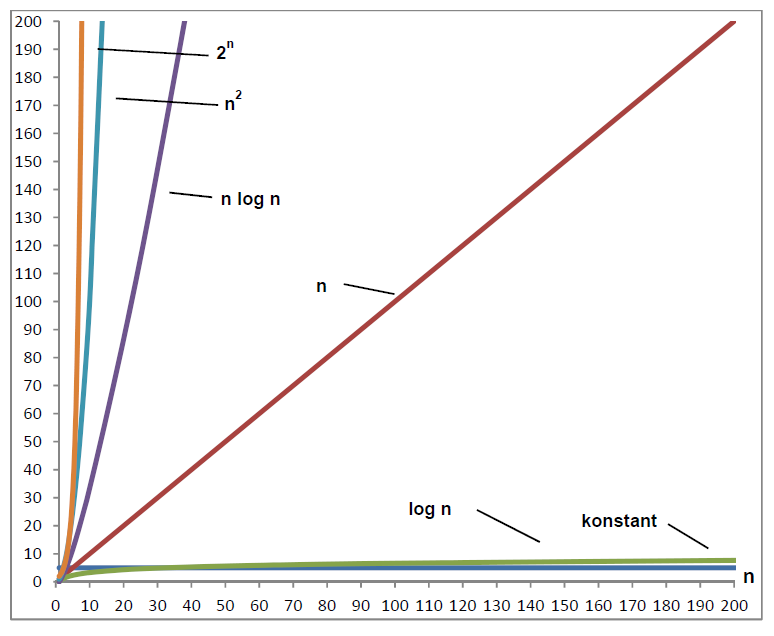
\includegraphics[width=0.5\textwidth]{images/Algorithmen/Wachstumsfunktionen.png}}
\label{Fig: Verschiedene Wachstumsfunktionen}
\end{center}
%------------------------------------------------------------------------------------------------



%------------------------------------------------------------------------------------------------
%Komplexitaetsklassen
%------------------------------------------------------------------------------------------------
\subsubsection{Komplexit"atsklassen}
DTM: Deterministische Turingmaschine, f"ur jeden Zustand bei gegebenem Input ist der n"achste Zustand eindeutig definiert. Ist praktisch realisierbar. \\
NTM: Nicht deterministische Turingmaschine, f"ur einen Zustand bei gegebenem Input ist der n"achste Zustand \textbf{nicht} eindeutig definiert. Heute noch nicht realisierbar, dient jedoch als Algorithmusausf"uhrungsmodell.\\
Folgende Klassen sind definiert:\\
\begin{itemize}
\item NL:       Von NTM auf logarithmischen Platz l"osbar 
\item P:        Von DTM in polynomialer Zeit l"osbar, $O(n^c)$
\item NP:       Von NTM in polynomialer Zeit lösbar, $O(n^c)$
\item PSPACE:   Von DTM auf polynomialem Platz l"osbar
\item EXPTIME:  Von DTM in exponentieller Zeit l"osbar, $O(2^n)$
\item EXPSPACE: Von DTM auf exponentiellem Platz l"osbar
\end{itemize}

Probleme der Klasse P lassen sich in vern"unftiger Zeit lösen. \\
Viele Probleme der Klasse NP lassen sich vermutlich nicht effizient l"osen.\\
Best"atigung oder Widerlegung dieses P-NP-Problems ist wohl das wichtigste offene Problem der Informatik.\\
Bekanntes NP-Problem ist das Travelling Salesman Problem.\\
%------------------------------------------------------------------------------------------------



%------------------------------------------------------------------------------------------------
%Suchalgorithmen
%------------------------------------------------------------------------------------------------
\subsection{Suchalgorithmen}
\subsubsection{Listensuche}
Finde Wert in einer Liste. 
\begin{lstlisting}[style=C]
int list[listLength];
int k;	//Zu findender Wert 				
int i; 	//Listenindex
\end{lstlisting} 
1. Art: Lineare Suche\\
Wenn nicht bekannt ist, ob die Liste irgendwie sortiert ist. \\
Komplexit"at: O(n)
\begin{lstlisting}[style=C]
for(i=0;i<listLength && k!=list[i];i++)
{}
found = i < listLength; 
\end{lstlisting} 

2. Art: Lineare Suche mit Sentinel\\
Beschleunigung des Codes durch Vereinfachung der Schleifenbedingung. Letztes Element wird durch gesuchtes Element ersetzt.\\
Die Schleife wird etwas schneller durchlaufen, aber die Komplexit"at ist noch immer O(n).
\begin{lstlisting}[style=C]
list[listLength-1] = k; //Sentinel setzen
for(i=0; k!= list[i]; i++)
{}
found = i < listLength-1; 
\end{lstlisting} 

3.Art: Bin"are Suche\\
Diese Suche funktioniert nur, wenn die Liste der Reihe nach sortiert ist.\\
Man geht von der Mitte der Liste aus, ist der gegebene Wert gr"osser als die Mitte sucht man in der oberen H"alfte auf dieselbe Art weiter, ansonsten in der unteren H"alfte.\\
Liegt der Wert am Rande ist die Suche auf diese Art erfolglos.\\
Komplexit"at: O(log(n))\\
\begin{lstlisting}[style=C]
left = 0; // Index des am weitesten links liegenden Kandidaten
right = listLength-1; // Index des am weitesten rechts liegenden Kandidaten
while (left <= right)
{
	pos = (left + right) / 2; // pos auf die mittlere Position setzen
	if (list[pos] == k)
		return pos;
	if (list[pos] > k)
		right = pos - 1;
	else
		left = pos + 1;
}
return -1; // nicht gefunden

\end{lstlisting} 
Siehe Beispiele im Skript 00-Algorithmen.pdf

\subsubsection{Mustersuche}
Ziel der Mustersuche: Ein ganzes Stringmuster (pattern) finden. Wenn man nur ein einzelnes Zeichen sucht, funktioniert dies wie bei der Listensuche oben.\\
1. Naiver Suchalgorithmus\\
Pattern wird zeichenweise am Text vorbei geschoben. Dies geschieht so lange bis das Pattern gefunden worden ist oder das Ende des Textes erreicht worden ist. Algorithmus wird ineffizient, wenn bis zum Schluss nichts gefunden worden ist.\\
Bei effizienteren Suchalgorithmen wird bei einer Nicht"ubereinstimmung nicht nur um ein Zeichen sondern um eine m"oglichst hohe Anzahl Zeichen geschoben. Die Intelligenz liegt hier beim Herausfinden dieser Anzahl.\\



\subsubsection{Sortieralgorithmen}
Je nach Form der vorliegenden Daten wird unterschieden zwischen: 
\begin{itemize}
\item Interne Sortierverfahren: Daten liegen im Hauptspeicher, auf die Daten besteht wahlfreier Zugriff (random access). Verfahren zum Sortieren von Feldern (Arrays).
\item Externe Sortierverfahren: Daten sind in Files auf externem Speicher, auf die Daten kann nur sequentiell zugegriffen werden. Sortieren von Files. 
\end{itemize}

Forderung an interne Sortierverfahren:\\
\begin{itemize}
\item Speicher: Algorithmus muss direkt mit dem Hauptspeicher auskommen. Kein Umkopieren, nur feste Anzahl von Hilfsvariabeln. In-Place-Algorithmen arbeiten direkt auf den Eingabedaten, Out-of-Place verwenden separate Ausgabedaten.
\item Effizienz: Um etwas "uber die Effizienz auszusagen werden vor allem die zwei f"ur das Sortieren wichtigen Operationen Comparison und Move betrachtet.
\item Stabilit"at: Ein stabiles Sortierverfahren ist ein Sortieralgorithmus, der die Reihenfolge der Datensätze, deren Sortierschlüssel gleich sind, bewahrt. (Wenn beispielsweise eine Liste alphabetisch sortierter Personendateien nach dem Geburtsdatum neu sortiert wird, dann bleiben unter einem stabilen Sortierverfahren alle Personen mit gleichem Geburtsdatum alphabetisch sortiert.)
\end{itemize}

Einfache Sortierverfahren:\\
1. Direktes Aussuchen (Straight Election)\\
Der unsortierte Teil wird nach dem kleinsten Element durchsucht, dieses wird dann mit dem ersten Element des unsortierten Teils vertauscht.\\
\begin{lstlisting}[style=C]
int i; // Laufvariable
int j; // Laufvariable
int k; // Index des kleinsten Elementes im nicht sortierten Teil
for (i = 0; i < listLength-1; ++i)
{
	k = i;
	for (j = i+1; j < listLength; ++j)
	{
		if (data[j] < data[k])
			k = j;
	}
	swap(i, k);
}
\end{lstlisting} 
Komplexit"at der Vergleiche: $O(n^2)$\\
Komplexit"at der Zuweisungen: $O(n)$\\

2. Direktes Einf"ugen (Straight Insertion)\\
Das erste unsortierte Element wird im sortierten Teil an die richtige Stelle gesetzt, alle gr"osseren sortierten Elemente m"ussen verschoben werden.
Ist effizient, wenn die Daten schon etwas sortiert sind. 
\begin{lstlisting}[style=C]
int i;
int j;
int buf; // Buffer
for (i = 1; i < listLength; ++i)
{
	buf = data[i];
	j = i;
	while (j > 0 && buf < data[j-1])
	{
		data [j] = data [j-1];
		j = j-1;
	}
	data[j] = buf;
}
\end{lstlisting} 
Komplexit"at der Vergleiche: $O(n^2)$\\
Komplexit"at der Zuweisungen: $O(n^2)$\\

3. Bubblesort\\
Benachbarte Elemente werden vertauscht, wenn sie nicht wie gew"unscht geordnet sind. Das relativ gr"osste Element steigt wie eine Blase im Wasser auf. 
\begin{lstlisting}[style=C]
int i;
int j;
for (i = listLength-1; i > 0; --i)
{
	for (j = 1; j <= i; ++j)
	{
		if (data[j-1] > data[j])
			swap(j-1, j);
	}
}
\end{lstlisting} 
Komplexit"at der Vergleiche: $O(n^2)$\\
Komplexit"at der Zuweisungen: $O(n^2)$\\

Schnelle interne Sortierverfahren:\\
1. Quicksort\\
Je gr"osser die Distanz beim Austauschen von Elementen ist, umso effizienter ist der Algorithmus. Dies nutzt Quicksort aus.\\
\textbf{Median}: Der Median einer Anzahl von Werten ist die Zahl, welche an der mittleren Stelle steht, wenn man die Werte nach Größe sortiert. Bsp: {4, 1, 37, 2, 1} Median = 2\\
Formale Beschreibung: \\
\begin{enumerate}
\item W"ahle ein beliebiges Pivot-Element aus (Median oder mittleres Element)
\item Laufe von linker Arraygrenze so lange nach innen, bis ein Element gefunden wird, welches \textbf{gr"osser gleich} das Pivot ist. 
\item Laufe von rechter Arraygrenze so lange nach innen, bis ein Element gefunden wird, welches \textbf{kleiner gleich} das Pivot ist. 
\item Vertausche die beiden Elemente
\item Wiederhole Schritt 2-4 so lange, bis sich die beiden Indizes getroffen haben
\item Das linke Teilfeld enth"alt nur noch Werte, die $\leq$ als das Pivot sind. Das rechte Teilfeld enth"alt nur noch Werte, die $\geq$ als das Pivot sind. 
\item Sortiere diese Felder wiederum rekursiv, bis nur noch Teilfelder mit einem einzigen Element "ubrig sind.
\end{enumerate}

\begin{lstlisting}[style=C]
void quickSort(int leftBound, int rightBound)
{
	int left = leftBound; // Index der linken Grenze
	int right = rightBound; // Index der rechten Grenze
	int pivot = data[(left+right) / 2]; // Gew"ahltes Element in der Mitte
	do
	{
		while (data[left] < pivot)
			left++;
		while (data[right] > pivot)
			right--;
		if (left <= right)
		{
			if (left < right)
				swap(left, right);
			left++;
			right--;
		}
	} while (left <= right);
	if (leftBound < right)
		quickSort(leftBound, right);
	if (rightBound > left)
		quickSort(left, rightBound);
}
\end{lstlisting} 
Bester Fall: Wenn als Pivot jedes mal der Median des Feldes getroffen wird $\rightarrow O(nlog(n))$\\
Schlechtester Fall: Wenn jedes Mal das Minimum oder Maximum getrofffen wird $\rightarrow O(n^2))$\\

Beispiel von Quicksort: \\
\begin{center}
{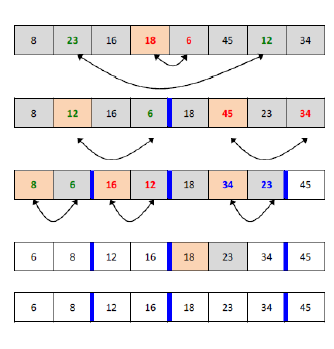
\includegraphics[width=0.5\textwidth]{images/Algorithmen/Quicksort.png}}
\label{Fig: Quicksort}
\end{center}

Wahl des Pivots ist wichtig. Ein Ansatz ist die median-of-3 Strategie, bei welcher der Median aus dem ersten, letzten und mittleren Element eines Bereiches gebildet und als Pivot verwendet. Bei b"osartig zusammengestellten Listen (median-of-3-killers) kann dies jedoch zu Problemen f"uhren.\\

\subsubsection{Effizienz verschiedener interner Suchalgorithmen}
\begin{tabular}{|c|c|c|c|c|}
\hline
Algorithmus & $C_{min}$ & $C_{ave}$ & $C_{max}$ & $O_C(\cdot)$ \\
\hline
Straight Selection & $\frac{n}{2}\cdot (n-1)$ & $\frac{n}{2}\cdot (n-1)$ & $\frac{n}{2}\cdot (n-1)$ & $n^2$ \\
\hline
Straight Insertion & $n-1$ & $\frac{1}{4}\cdot (n^2 + 3n -4)$ & $\frac{1}{2}\cdot (n^2+n-2)$ & $n^2$ \\
\hline
Bubblesort & $\frac{n}{2}\cdot (n-1)$ & $\frac{n}{2}\cdot (n-1)$ & $\frac{n}{2}\cdot (n-1)$ & $n^2$ \\
\hline
Quicksort & $n\cdot ld(n)$ & $2\cdot n \cdot ln(n)$ & $\frac{1}{2}\cdot (n+3)(n+2)-10$ & $n^2$ \\
\hline
\end{tabular}

\subsubsection{Systemfunktionen f"ur Suchen und Sortieren}
Siehe Skript 00-Algorithmen.pdf S.25